\secput{example}{Example}

Assuming we have input bit-matrix as follows ($3$ rows, $5$ columns):

\[ 
\begin{pmatrix} 
0 & 0 & 0 & 1 & 1 \\
0 & 0 & 1 & 0 & 1 \\
0 & 1 & 0 & 0 & 1 \\
\end{pmatrix}
\]

So it has $5$ input columns, $g = 3$.

After stage $1$, it has following bins:

\begin{figure}[!h]
\begin{minipage}[b]{0.5\linewidth}
\centering
\begin{tabular}{|c|ccccc|}
\hline
bin 1 & column 0 & column 1 & column 2 & column 3 & column 4 \\
\hline
00x & 1 & 1 & $\infty$ & $\infty$ & $\infty$ \\
0x0 & 1 & $\infty$ & 1 & $\infty$ & $\infty$ \\
x00 & 1 & $\infty$ & $\infty$ & 1 & $\infty$ \\
\hline
bin 2 & column 0 & column 1 & column 2 & column 3 & column 4 \\
\hline
0xx & 2 & 2 & 2 & $\infty$ & $\infty$ \\
x0x & 2 & 2 & $\infty$ & 2 & $\infty$ \\
xx0 & 2 & $\infty$ & 2 & 2 & $\infty$ \\
xx1 & $\infty$ & 2 & $\infty$ & $\infty$ & 2 \\
x1x & $\infty$ & $\infty$ & 2 & $\infty$ & 2 \\
1xx & $\infty$ & $\infty$ & $\infty$ & 2 & 2 \\
\hline
bin 3 & column 0 & column 1 & column 2 & column 3 & column 4 \\
\hline
xxx & 3 & 3 & 3 & 3 & 3 \\
\hline
\end{tabular}
\caption{Generated data structure in bins}
\label{fig:bin}
\end{minipage}
\hspace{0.2cm}
\begin{minipage}[b]{0.5\linewidth}
\centering
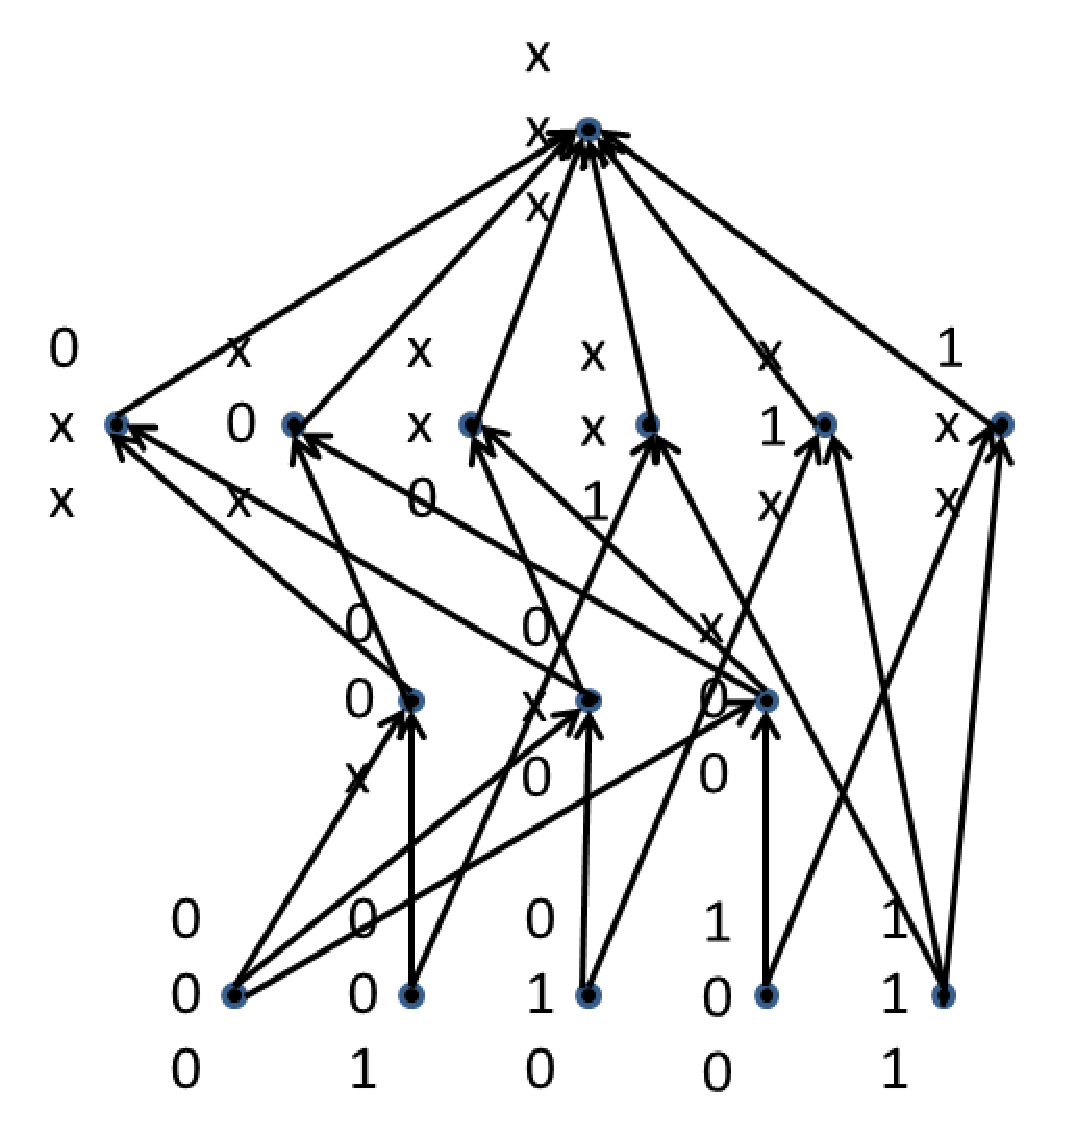
\includegraphics[scale=0.5]{figures/dag.eps}
\caption{Generated {DAG} data structure}
\label{fig:dag}
\end{minipage}
\end{figure}

From ~\figref{bin}, we can see that from $5$ input columns, the algorithm will
generate $10$ new nodes spreaded in $3$ different bins.  If including
the input $5$ columns, the {DAG} has $15$ total nodes as illustrated
in \figref{dag}.
